\documentclass[11pt, oneside]{article}
\usepackage{geometry}
\geometry{a4paper, top=0mm,left=20mm,right=20mm,bottom=18mm}
\usepackage[parfill]{parskip} %newline for paragraphs
\usepackage{url}
\usepackage{listings}
\usepackage{graphicx}
\usepackage{multicol}
\usepackage{caption}

\usepackage{lipsum}
\newenvironment{Figure}
  {\par\medskip\noindent\minipage{\linewidth}}
  {\endminipage\par\medskip}
%\usepackage{savetrees}

\title{COMS20001 - Concurrent Computing - Coursework 1}
\author{\textbf{map} ("Adam " ++) ["Beddoe", "Fox"]   |  ab16301/af16371 }
\date{\vspace{-5mm}}

\begin{document}
\maketitle

\section{Functionality \& Design}
The xCore-200 eXplorerKIT implementation of John Horton Conway's Game-of-Life implements the following functionality:

\begin{itemize}
\setlength\itemsep{-2mm}
	\item Correctly evolving Game-of-Life, according to the given rules
	\item 2, 4 or 8 worker threads
	\item Button, board orientation and LED behaviour
	\item Ability to process larger than 512x512 images with memory on both tiles
	\item Timers to measure processing speed and comprehensive unit testing
	\item Ability to generate \& process random images up to a size of 1472x1472 on the board
        \item Dynamically chooses implementation based on input size
\end{itemize}

\vspace{-4mm}
\subsection{Method}
\vspace{-2mm}
In order to iterate the game of life, the program works as follows: The main function starts up all threads, specifies which tiles they are on, and assigns channels between them. The distributor function is responsible for mechanics such as LED behaviour, accelerometer pausing and instructing the workers to input and output the current game state. To minimise thread communication, the workers pass board state directly to the IO threads when required and only communicate with the distributor to send a confirmation signal each round and to send the count of live cells when the game is paused. The workers remain in sync as they require synchronous communication to share columns each round.


\vspace{-4mm}

\subsection{Worker Types}
\vspace{-2mm}
Each of the worker threads receives an equal column of the total image. There are two different worker systems, the program dynamically chooses the best implementation based on the size of the input image:

\vspace{-4mm}
\subsubsection{Unpacked Worker}
\vspace{-3mm}

This worker reads in the segment of the image it is passed from the IO stream and stores it in a uchar array, where each element can be 1 or 0 and represents an alive or dead cell respectively. An extra column on each side stores the state of left and right worker's outmost columns. The threads communicate in pairs, passing or receiving first depending on whether they have an odd or even ID. They then proceed to make a copy of the array, and iterate on the original, based on the sum of the neighbours of each square. The additional columns mean that the solution requires no further communication until the next round. It will then continue iterating and communicating with the adjacent threads until told to perform one of the IO actions by the distributor.

\vspace{-4mm}
\subsubsection{Packed Chunk Worker}
\vspace{-3mm}

This implementation uses bit packing, and splitting the image up into chunks, making it optimal for reduced memory usage. This allows for large images, in this case up to 1472x1472.
Packing into an unsigned char (uchar) it is possible to store 8 values in each, drastically reducing the memory required but adding computational complexity by computing the packing and unpacking, and the copying of edges between chunks each round. The \emph{left, right, top, bottom} variables hold the corresponding edge of the neighbouring chunk and the 4 most significant bits in \emph{corners} store the 4 adjacent corners. The storing of the neighbours for each chunk rather than the whole array means that the base array takes up more space, however only one chunk needs to be loaded into memory when iterating, rather than making a copy of the entire worker's array.


\newgeometry{top=20mm,left=20mm,right=20mm,bottom=20mm} 
\pagebreak
\section{Tests \& Experiments}
\subsection{Packed vs. Unpacked}
In order to see which of the approaches is faster, the differing speeds of iteration were measured while changing three main parameters: Packed/Unpacked implementation, number of worker threads and size of image. Below is the data collected (values in seconds): 


\begin{center}
No of threads
\end{center}

\begin{table}[!th]
\centering
Image size
\begin{tabular}{l|lll}
    & 2        & 4        & 8        \\ \hline
16  & 0.029248 & N/A      & N/A      \\
64  & 0.461743 & 0.233838 & 0.190104 \\
128 & 1.839617 & 0.918425 & 0.74095  \\
256 & 7.08548  & 3.548166 & 2.81206 
\end{tabular}
\captionof{table}{Unpacked Worker}
\end{table}

\vspace{4mm}

\begin{center}
No of threads
\end{center}

\begin{table}[!th]
\centering
\label{my-label}
Image size
\begin{tabular}{l|lll}
    & 2          & 4         & 8        \\ \hline
16   & 0.036808   & N/A       & N/A      \\
64   & 0.61281    & 0.30677   & 0.227792 \\
128  & 2.447382   & 1.223531  & 0.972146 \\
256  & 9.756354   & 4.853463  & 3.880383 \\
512  & 39.461591  & 19.442143 & 15.49954 \\
1024 & 152.395147 & 77.946608 & 62.25204
\end{tabular}
\caption{Packed worker}
\end{table}

\pagebreak
\subsection{Graphs}

\begin{Figure}
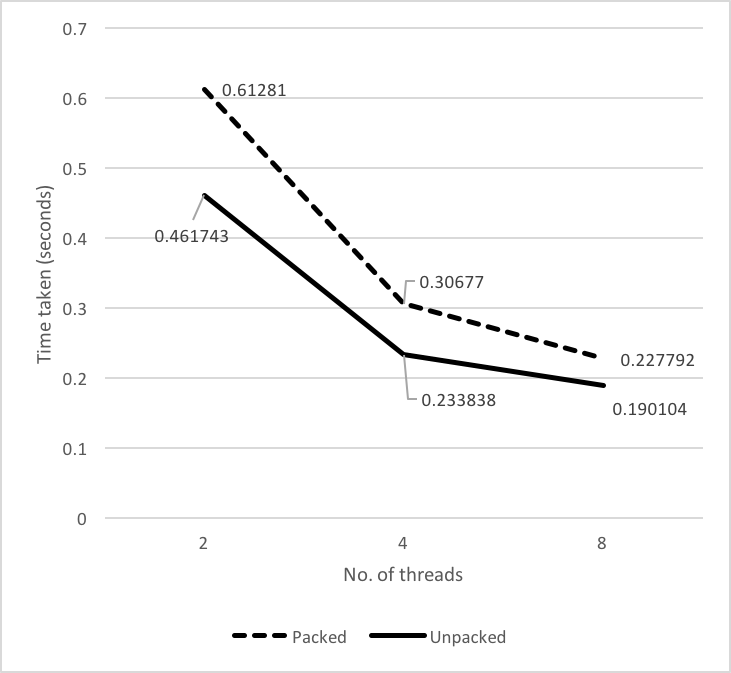
\includegraphics[width=9cm]{images/64x64graph.png}
\captionof{figure}{16x16}
\end{Figure}



\subsection{2 Round Images}
As required, below are the second round images for all of the provided example images. Additionally, \emph{Figure 6} is an example of the largest possible image (1472x1472).

\begin{multicols}{3}

%column1
\begin{Figure}

\includegraphics[width=\linewidth]{images/16x16_2_1.png}
\captionof{figure}{16x16}
\end{Figure}

\begin{Figure}
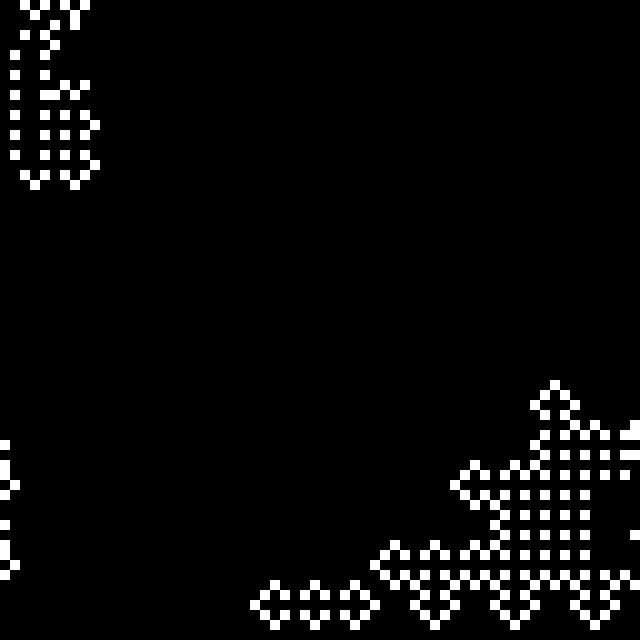
\includegraphics[width=\linewidth]{images/64x64_2_1.png}
\captionof{figure}{64x64}
\end{Figure}


%column2
\begin{Figure}
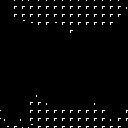
\includegraphics[width=\linewidth]{images/128x128_2.png}
\captionof{figure}{128x128}
\end{Figure}

\begin{Figure}
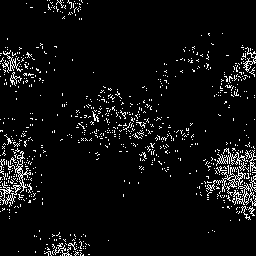
\includegraphics[width=\linewidth]{images/256x256_2.png}
\captionof{figure}{256x256}
\end{Figure}


%column3
\begin{Figure}
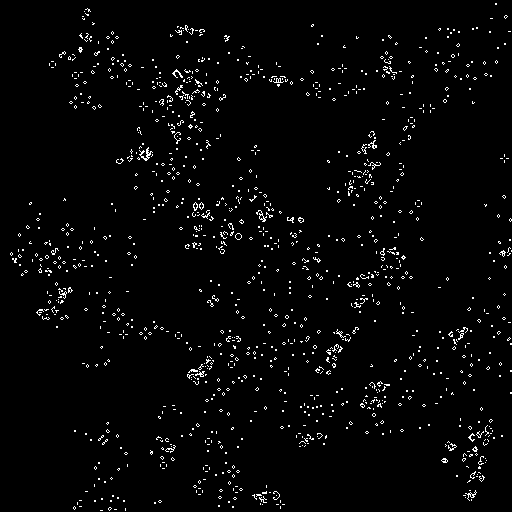
\includegraphics[width=\linewidth]{images/512x512_2.png}
\captionof{figure}{512x512}
\end{Figure}

\begin{Figure}

\includegraphics[width=\linewidth]{images/1472x1472.png}
\captionof{figure}{1472x1472}
\end{Figure}

\end{multicols}



\pagebreak
\section{Critical Analysis}
Through testing, it was determined that the additional time complexity of packing and unpacking meant that the



\bibliographystyle{unsrt}
\bibliography{}
\end{document}
